%!TEX root = main.tex

%\revision{
\subsubsection{Semantics of $\FOAMASS$}\label{sec-foamass}
In this case, we assume that there is only one activity $A_0$ and consider the fragments as the atomic objects, hence we only consider the transaction rules $\back$ , $A\xrightarrow{\mu}T$ and $F\xrightarrow{\mu}T$, where $T$ is of the form $(\beta_1(F_1, i_1, x_1), \cdots, \beta_k(F_k, i_k, x_k))$ such that for every $j \in [k]$, $\beta_j \in \{\ADD, \REP, \REM\}$, $F_j \in \frag$, $i_j \in \Nn$, and $x_j$ is a variable storing the identifiers of fragment instances.
%}

\subsection*{Intuitions.}
The intuitions of the transition rules  $A\xrightarrow{\mu}T$ and $F\xrightarrow{\mu}T$ are explained in the sequel. 
\begin{itemize}
	\item 
	$\ADD(F, i,  x)$ denotes the action where a \emph{new} instance of the fragment $F$ is added to the container $i$ of the current activity. Moreover, the identifier of the new instance is stored in $x$.
	
	\item $\REP(F, i,  x)$ is the same as $\ADD(F, i,  x)$, except that the container %of identifier 
	$i$ is cleared before adding $F$. 
%
	\item $\REM(F, i,  x)$ denotes the action where the instance of the fragment $F$ of the identifier (stored in) $x$ is removed from the container $i$ of the current activity.	 
	
\item $\opstack[(\beta_1(F_1, i_1, x_1), \cdots, \beta_k(F_k, i_k, x_k))]$ denotes that the actions $\beta_1(F_1, i_1, x_1),\cdots, \beta_k(F_k, i_k, x_k)$ are executed sequentially, and %$(\beta_1(F_1, i_1), \cdots, \beta_k(F_k, i_k))$ is
	are added to the transaction stack. 
\item $\nopstack[(\beta_1(F_1, i_1, x_1), \cdots, \beta_k(F_k, i_k, x_k))]$ is the same as $\opstack$, except that %$(\beta_1(F_1, i_1), \cdots, \beta_k(F_k, i_k))$
	the transactions will \emph{not} be added to the transaction stack. \\
	For convenience, these transition rules are called $\opstack$-transition rules and $\nopstack$-transition rules respectively.
\end{itemize}

It is fair to say that the intricacy of the semantics lies in the action $\back$. Let $A$ be the top activity of the top task, %$\vgr(A)=(i_1, \cdots, i_m)$, and $\upsilon = ((V_1, i_1), \cdots, (V_m, i_m))$ be an enumeration of the fragment stacks corresponding to the containers (where $V_j \in \frag^*$ for every $j \in [m]$), 
$\vgr(A)=(i_1, \cdots, i_m)$, $V_{1}$, $\cdots$, $V_{m}$ be the fragment stacks for the containers $i_1, \cdots, i_m$,  
%where each $V_i$ is a fragment stack 
and $\eta \in \ops^*$ be the transaction stack. 
If $\eta = \epsilon$, the activity $A$ will be popped, otherwise the behavior of the action $\back$ is controlled by $\eta$, namely, when the back button is pressed, the top transaction of $\eta$ is removed from $\eta$ and its effects on the fragment stacks %$\upsilon$ are canceled
are to be revoked. Noticeable difficulties arise.  %Canceling the effects of an transaction is intricate in the following two aspects: 

\smallskip
\noindent\emph{Mismatch between fragment and transaction stack.} 
The transaction stack $\eta$ may \emph{not} contain all the historical transactions leading to the fragment stacks, but only those corresponding to the $\opstack$-transition rules, which means that when revoking the top action of $\eta$, say $\ADD(F, i_j, x_j)$, $F$ may not be the top fragment of $V_j$. To deal with this issue, we 
\begin{enumerate}
\item store $(F, n)$ in $V_{j}$, where $n$ is the identifier of the instance of $F$ which is generated when applying $\ADD(F, i_j, x_j)$,  
\item store the concretized action $\ADD(F, i_j, n)$, instead of $\ADD(F, i_j, x_j)$, into the transaction stack $\eta$.
\end{enumerate}
As a result, we can revoke $\ADD(F, i_j, n)$ instead of $\ADD(F, i_j, x_j)$ in the transaction stack, and use $n$ to identify the fragment instance to be removed from the fragment container $V_j$.
%
%Note that when revoking $\ADD(F, i_j, x_j)$, the variable $x_j$ cannot be used to find the fragment instance since $x_j$ since $x_j$ may have been reused to store the identifiers of the other fragment instances.

\smallskip
\noindent\emph{Revoking $\REP$ actions.} The top transaction of $\eta$ may include some action $\REP(F, i_j, n)$ and revoking these actions requires restoring the historical content of the container $i_j$ before applying this action.

%To deal with the first issue, %mismatch between $\upsilon$ and $\eta$, 
%when defining the formal semantics in the sequel, the tag $\sharp$ is used 
%we use a tag $\sharp$ to distinguish between the fragment instances added by the $\opstack$-transition rules and those added by the $\nopstack$-transition rules. When applicable, pairs $(F, \sharp)$, instead of fragments $F$,  are pushed into the fragment stack. %container.

%To deal with the second issue, %the canceling of $\REP$ actions, 
%we introduce a new action $\REM(F', i_j)$ where $F' \in \frag \cup (\frag \times \{\sharp\})$, whose meaning is to remove the topmost occurrence of $F'$ from the container $i_j$. 
%
To deal with this issue, 
when an action $\REP(F, i_j, x_j)$ appears in a $\opstack$-transition rule and is to be pushed into the transaction stack, suppose that the current content of the container $i_j$ is $((F'_1,n'_1),  \cdots, (F'_k, n'_k))$, then $\REP(F, i_j, x_j)$ is concretized into the action sequence 
$$\REM(F'_1, i_j, n'_1), \cdots, \REM(F'_k, i_j, n'_k), \ADD(F, i_j, n),$$ 
which---instead of $\REP(F, i_j, n)$---is pushed into the transaction stack, possibly together with the other actions in the same transaction. 
(Note that $n$ is the identifier of the newly created instance of $F$.)
Hence revoking $\REP(F, i_j, x_j)$ is to apply the concretized actions
%the inverse of the action sequence $\REM(F'_1, j), \cdots, \REM(F'_k, j), \ADD((F,\sharp), j)$, namely, 
$\REM(F, i_j, n), \ADD(F'_k, i_j, n'_k), \cdots, \ADD(F'_1, i_j, n'_1)$ one by one.

Therefore, only concretized actions of the form $\ADD(F, i, n)$ or $\REM(F, i, n)$ are stored in the transaction stack, and we use $\cops$ to denote the set of these concretized actions.  



\subsection*{Fragment containers and configurations.}
%
%Let $\frag^\sharp = \frag \times \{\sharp\}$. 
%,  where the tag $\sharp$ is introduced for encoding the semantics of the action $\back$ and will be explained later on.
 
A \emph{fragment \container} is encoded as 
$$V = ((F_1, n_1), \cdots, (F_k, n_k)) \in (\frag \times \Nn)^+ ,$$ where $n_j$ is the identifier of an instance of $F_j$ for $j \in [k]$ and $k$ is called the \emph{height} of $V$.

%
A \emph{configuration} $\rho$ %with {\container} $\vgr(A) = (V_1, \cdots, V_m)$ 
is encoded as a tuple $(\upsilon, \eta, \iota)$, where %$\upsilon = ((V_1, i_1), \cdots, (V_m, i_m))$ such that $V_j \in (\frag\cup \frag^{\sharp})^+$ is the corresponding fragment stack  to $i_j$, and 
$\upsilon = (V_1, \cdots, V_m)$  is a sequence of fragment containers associated with $A_0$, where $\vgr(A_0) = (i_1,\cdots,i_m)$, $\eta= (T_1, \cdots, T_n) \in \cops^*$ is the transaction stack, and $\iota$ is the assignment function that assigns to each variable $x$ in $\Mm$ an identifier, i.e. a natural number. Note that it is possible that $m=0$ and/or $n=0$. For technical convenience, let $\iota_0$ denote the assignment function that assigns each variable $x$ the value $0$. The initial configuration of $\Mm$ is $((\epsilon,\cdots,\epsilon),\epsilon,\iota_0)$.

%%%%%%%%%%%%%%%%%%%%%%%%%%%%%%%%%%%%%%%%%%%%%%%%%%%%%%%%%%%%%%%%%%
%%%%%%%%%%%%%%%%%%%%%%%%%%%%%%%%%%%%%%%%%%%%%%%%%%%%%%%%%%%%%%%%%%
\subsection*{Auxiliary functions and predicates.} To specify the transition relation precisely and concisely, we define the following functions and predicates. 
For a container $V=((F_1, n_1), \cdots, (F_{m}, n_m))$, define $\tfrag(V) = F_1$.
%For $\rho_v = (V_1,\dots,V_n)$, $\rho_o = (O_1,\dots,O_n)$, $\vec{\beta} = [\beta_1(F_1',V_1),\dots,\beta_m(F_m',V_m)]$
%\begin{itemize}
%	\item   $\tfrag(V) = F_1$,  
	%
%		\item $\getfrag(F, V) = \min\{1\leq i\leq m  \mid F = F_i\}$ and we write $\bot$ for $\min\emptyset$. $\getfrag(F, V)$ returns the first (topmost) instance of $F$ in $V$. 
		%otherwise, $\getfrag(F, V) = \bot$. (Intuitively, $\getfrag(F, V)$ returns the index of the first occurrence of $F$ in $V$.)
%	\item  If there is $i \in [m]$ such that $F = F_i$ and for every $ j \in [i-1], F_j \neq F$, then $\getfrag(F, V) = i$; otherwise, $\getfrag(F, V) = \bot$. (Intuitively, $\getfrag(F, V)$ returns the index of the first occurrence of $F$ in $V$.)
%\end{itemize}

Let $\rho = (\upsilon, \eta, \iota)$ be the configuration of associated with $A_0$, where $\vgr(A_0) = (i_1, \cdots, i_k)$  ($k > 0$), $\upsilon = (V_1, \cdots, V_k)$ is the container sequence, and $\eta = (T_1, \cdots, T_l)$ ($l \ge 0$) is the transaction stack. Moreover, let $F \in \frag$, $j \in [k]$, and $x$ be a variable. 
We define the following functions.

%Then we define the following functions manipulating containers.
%For $\rho_v = (V_1,\dots,V_n)$, $\rho_o = (O_1,\dots,O_n)$, $\vec{\beta} = [\beta_1(F_1',V_1),\dots,\beta_m(F_m',V_m)]$
\begin{itemize}
\item %For a container $V=(F'_1, \cdots, F'_{m'})$, define $\tfrag(V) = F'_1$. Moreover, 
$\tfrag(\upsilon) = \{\tfrag(V_i) \mid i \in [k], V_i \neq \epsilon\}$ returns the set of topmost fragments of containers in $\upsilon$.
%
%\item  For a container $V=(F'_1, \cdots, F'_{m'})$, define $\getfrag(F', V)$ as follows: If there is $i \in [m']$ such that $F' = F'_i$ and for every $ j \in [i-1], F'_j \neq F'$, then $\getfrag(F', V) = i$.
%        Otherwise, $\getfrag(F', V) = \bot$.
%
\item  $\ADD(F, i_j, x)(\upsilon, \iota) = (\upsilon', \iota')$, where $\upsilon' = (V_1, \cdots, V_{j-1}, (F, n) \cdot V_j, V_{j+1}, \cdots, V_k)$, $\iota' =\iota[n/x]$,  and $n$ is the \emph{minimum} identifier not occurring in $\upsilon$ or $\iota$. Intuitively, $\ADD(F, i_j, x)(\upsilon, \iota)$ updates $(\upsilon, \iota)$ by choosing a fresh identifier $n$, pushing $(F, n)$ into the container $i_j$, and storing $n$ into $x$. 
%    otherwise, 
%    $$(\ADD(F', i))(\upsilon) = (((F'), i'), (V_1, i_1), \cdots, (V_k, i_k)).$$
%
 \item $\REP(F, i_j, x)(\upsilon, \iota) =  (\upsilon', \iota')$, where $\upsilon' = (V_1, \cdots, V_{j-1}, (F, n), V_{j+1}, \cdots, V_k)$, $\iota' = \iota[n/x]$, and $n$ is the \emph{minimum} identifier not occurring in  $\upsilon$ or $\iota$. Intuitively, $\REP(F, i_j, x)(\upsilon, \iota)$ updates $\upsilon$ by replacing the content of container $i_j$ with $(F, n)$, and storing $n$ into $x$.
    %
%    otherwise, 
    %
%    $$(\REP(F',i'))(\upsilon) = (((F'), i'), (V_1, i_1), \cdots, (V_k, i_k)).$$
%
\item Suppose $V_j = ((F_1, n_1), \cdots, (F_{m}, n_m))$, then
%
$\REM(F, i_j, x)(\upsilon, \iota) = (\upsilon', \iota')$, 
%
where 
\begin{itemize}
\item $\upsilon' = (V_1, \cdots, V_{j-1}, \tilde{V}$, $V_{j+1}, \cdots, V_k)$ such that
\begin{itemize}
\item $\tilde{V} = V_j$,  if $\iota(x) \neq n_{j'}$ for every $j' \in [m]$, and 
\item $\tilde{V} = ((F_1,n_1), \dots, (F_{l-1}, n_{l-1}), (F_{l+1}, n_{l+1}), \dots, (F_{m}, n_m))$, if $\iota(x) = n_l$, 
\end{itemize}
\item moreover, $\iota' = \iota$.
\end{itemize}

Intuitively, the action $\REM(F, i_j, x)(\upsilon)$ updates $\upsilon$ by removing the instance of $F$ of the identifier $\iota(x)$ from container $i_j$ and does not change $\iota$.
%
\item Furthermore, the functions $\ADD(F, i_j, n)(\upsilon, \iota)$, $\REP(F, i_j, n)(\upsilon, \iota)$, $\REM(F, i_j, n)(\upsilon, \iota)$ for concretized actions can be defined similarly (except that $\iota$ is unchanged).
\end{itemize}

For a  transaction $T=(\beta_1(F_1, j_1, x_1), \cdots, \beta_{r}(F_r, j_r, x_r))$ such that $\beta_s \in \{\ADD,\REM,\REP\}$ and $F_s \in \frag$ for every $s \in [r]$, 
 $\updateviews_T(\upsilon, \iota)= (\upsilon_r, \iota_r)$, where $(\upsilon_0, \iota_0) = (\upsilon, \iota)$, and for every $s \in [r]$, $(\upsilon_s, \iota_s) = \beta_s(F_s, j_s, x_s)(\upsilon_{s-1}, \iota_{s-1})$, i.e. $\updateviews_T$ updates the containers and the assignment function by applying the actions in $T$. Furthermore, $\updateviews_T(\upsilon, \iota)$ can be defined similarly for concretized transactions $T$.


%\begin{itemize}
    %(Note in $O^{-1}$, the sequence $\beta_1, \cdots, \beta_r$ is reversed and $\sharp$ is added.)
    %
%    \item For an transaction $O=(\beta_1(F'_1, j_1), \cdots, \beta_{r}(F'_r, j_r))$ such that $\beta_s \in \{\ADD,\REM\}$ and $F'_s \in \frag \cup \frag^\sharp$ for every $s \in [r]$ (note here $\beta_s \neq \REP$), 
%    
  
%\item   $\updateviews_T(\upsilon, \iota)= (\upsilon_r, \iota_r)$, where $(\upsilon_0, \iota_0) = (\upsilon, \iota)$, and for every $s \in [r]$, $(\upsilon_s, \iota_s) = \beta_s(F_s, j_s)(\upsilon_{s-1}, \iota_{s-1})$, i.e. $\updateviews_T$ updates the containers and the assignment function by applying the actions in $T$, 
%
%\item if $F_1, \cdots, F_r \in \frag$, then $\updateviews^\sharp_T(\upsilon, \iota)= (\upsilon_r, \iota')$, where $\upsilon_0 = \upsilon$, and for every $s \in [r]$, 
%$(\upsilon_s, \iota_s) = \beta_s((F_s,\sharp), j_s)(\upsilon_{s-1}, \iota_{s-1})$, i.e. $\updateviews^\sharp_T$ updates the containers by applying the $\sharp$-decorated actions in $T$, 
%
%\item   $T^{-1} = (\beta^{-1}_r(F_r, j_r), \cdots, \beta^{-1}_{1}(F_1, j_1))$ is the dual transaction of $T$.
%\end{itemize}

We also introduce a function that concretize the actions $\REP$ by utilizing the containers in $\upsilon$. Suppose $F \in \frag$, $j \in [k]$, $x$ is a variable, and $V_j = ((F_1, n_1), \cdots, (F_{m}, n_m))$. Let $n$ be the minimum identifier not occurring in $\upsilon$ or $\iota$.
% \begin{itemize}
%\item 
Then
$$
%\begin{array}{l}
\concaction_{\upsilon, \iota}(\REP(F, i_j, x)) =
%\ \ \ \ 
\REM(F_{1}, i_j, n_1), \cdots, \REM(F_{m}, i_j, n_m), \ADD(F, i_j, n).
%\end{array}
$$
%where $n$ is the minimum identifier not occurring in $\Theta$.
%
%
Moreover, let 
$$\concaction_{\upsilon,\iota}(\ADD(F, i_j, x)) = \ADD(F, i_j, n) \mbox{ and } \concaction_{\upsilon,\iota}(\REM(F, i_j, x)) = \REM(F, i_j, \iota(x))$$
by convention.
%
%\item $\concaction^\sharp_\upsilon(\ADD(F, i_j))$ and $\concaction^\sharp_\upsilon(\REP(F, i_j))$ are defined similarly, with $F$ replaced by $(F, \sharp)$,
%

Let $T = (\beta_1(F_1, j_1, x_1), \cdots, \beta_k(F_r, j_r, x_r))$ be a transaction such that $\beta_s \in \{\ADD,\REM, \REP\}$, and $F_s \in \frag$ for every $s \in [r]$.
We define $\concaction_{\upsilon, \iota}(T)$ as the concatenation of the concretized action sequences 
$ \concaction_{\upsilon_0, \iota_0}(\beta_1(F_1, j_1, x_1))$, $\cdots$, $\concaction_{\upsilon_{s-1}, \iota_{s-1}}(\beta_s(F_s, j_s, x_s))$,
where $(\upsilon_0, \iota_0)= (\upsilon, \iota)$, and for each $s \in [r]$, $(\upsilon_s, \iota_s) = \beta_s(F_s, j_s, x_s)(\upsilon_{s-1}, \iota_{s-1})$.

Finally, we define functions $\beta^{-1}(F, i_j, n)$ for $\beta(F, i_j, n) \in \cops$ as follows.
\begin{itemize}
 \item $\ADD^{-1}(F, i_j, n)(\upsilon, \iota) =\REM(F, i_j, n)(\upsilon, \iota)$,
 \item $\REM^{-1}(F, i_j, n)(\upsilon, \iota) = \ADD(F, i_j, n)(\upsilon, \iota)$.
\end{itemize}
Intuitively, $\ADD(F, i_j, n)$ and $\REM(F, i_j, n)$ are dual actions.
%
Moreover, for a concretized transaction 
$$T = (\beta_1(F_1, j_1, n_1), \cdots, \beta_{r}(F_r, j_r, n_r))$$ 
such that $\beta_s \in \{\ADD,\REM,\REP\}$, $F_s \in \frag$ for every $s \in [r]$, and $n \in \Nn$, we define $T^{-1}$ as 
$$(\beta^{-1}_{r}(F_r, j_r, n_r), \cdots, \beta^{-1}_1(F_1, j_1, n_1)).$$



%===============================================================================================================	
\subsection*{Transition relation.} 
We assume that the current activity is $A$. For $\rho\xrightarrow[\tau]{\Mm}\rho'$, we let $\rho = (\upsilon,\eta,\iota)$ be the current configuration, where
$\vgr(A) = (i_1, \cdots, i_k)$, 
$\upsilon = (V_1, \cdots, V_k)$, and $\eta = (T_1, \cdots, T_l)$.
\begin{itemize}
    \item If $\tau = \back$, then we assume that $\eta\neq\epsilon$, otherwise $A$ will be popped and there is no activity to store fragments. Then $\rho' = (\upsilon',\eta',\iota')$, where $(\upsilon', \iota') = \updateviews_{T_1^{-1}}(\upsilon, \iota)$, and $\eta' = (T_2, \cdots, T_l)$.  Note that $T_1$ is popped off the transaction stack and the actions of $T_1$ are revoked on $(\upsilon, \iota)$.
    \item If $\tau = A\xrightarrow{\mu}T$, or $\tau = F\xrightarrow{\mu}T$, and $F\in\topfrag(\upsilon)$
    we let 
    $$T = (\beta_1(F_1, i_1, x_1), \cdots, \beta_k(F_k, i_k, x_k)),$$ then $\rho' = (\upsilon',\eta',\iota')$ is obtained from $\rho$ by applying all the actions in $T$ to the containers and assignment function, such that $(\upsilon', \iota') = \updateviews_{T}(\upsilon, \iota)$ and $\eta' = \concaction_{\upsilon, \iota}(T) \cdot \eta$ if $\mu = \opstack$, $\eta' = \eta$ otherwise.
    Note that the difference between $\opstack$ and $\nopstack$ is that the concretization of $T$ is stored into the transaction stack when $\mu=\opstack$.
\end{itemize}

We use the following example to illustrate the formal semantics of $\FOAMASS$.
\begin{example}\label{exam:frag-amass}
    Let $\Mm = (\act,A_0,\frag,\lmd,\aft,\vgr, \Delta)$ be a {$\FOAMASS$}, where $\act = \{A_0\}$, $\frag = \{F_1,F_2,F_3\}$, and $\vgr(A_0) = (1)$.
    Moreover, $\Delta =\{\back\} \cup \{\tau_i \mid 0 \le i \le 3\}$, where
    % $\rho_0 = (([D_1],D_1,1))$, and\\
        $\tau_0 = \back$,
        $\tau_1 = F_1\xrightarrow{\opstack}(\ADD(F_2,1,x))$,
        $\tau_2 = F_2\xrightarrow{\nopstack}(\REP(F_3,1,x))$, and
        $\tau_3 = F_3\xrightarrow{\nopstack}(\REM(F_3,1,x))$.
Then the relation $\xrightarrow{\Mm}$ on the set of configurations that are reachable from the initial configuration $(([(F_1,0)]),\epsilon,\{x=0\})$ is illustrated in Figure~\ref{frg-example}. 

For instance, 
\begin{itemize}
            \item from the configuration $(([(F_1,0)]),\epsilon,\{x=0\})$, after executing the transition rule $F_1\xrightarrow{\opstack}(\ADD(F_2,1,x))$, we have 
            $$(\upsilon', \iota') = \updateviews_{T}(\upsilon, \iota) = \ADD(F_2,1,x)([(F_1,0)],\{x=0\})=([(F_2,1)(F_1,0)], \{x=1\}),$$ 
            $$\eta' = \concaction_{\upsilon, \iota}(T) \cdot \eta = \concaction_{\upsilon, \iota}(\ADD(F_2,1,x)) = \ADD(F_2,1,1),$$
            % \item from the configuration $(([(F_1,0)]),\epsilon,\{x=1\})$, after executing the transition rule $F_1\xrightarrow{\opstack}(\ADD(F_2,1,x))$, we have 
            % $$(\upsilon', \iota') = \updateviews_{T}(\upsilon, \iota) = \ADD(F_2,1,x)([(F_1,0)],\{x=1\})=([(F_2,2)(F_1,0)], \{x=2\}),$$ 
            % $$\eta' = \concaction_{\upsilon, \iota}(T) \cdot \eta = \concaction_{\upsilon, \iota}(\ADD(F_2,1,x)) = \ADD(F_2,1,2),$$
            % \item from the configuration $(([(F_1,0)]),\epsilon,\{x=0\})$, after executing the transition rule $F_1\xrightarrow{\opstack}(\ADD(F_2,1,x))$, we have 
            % $$(\upsilon', \iota') = \updateviews_{T}(\upsilon, \iota) = \ADD(F_2,1,x)([(F_1,0)],\{x=2\})=([(F_2,1)(F_1,0)], \{x=1\}),$$ 
            % $$\eta' = \concaction_{\upsilon, \iota}(T) \cdot \eta = \concaction_{\upsilon, \iota}(\ADD(F_2,1,x)) = \ADD(F_2,1,1),$$
            \item from the configuration $(([(F_2,1),(F_1,0)]),[(\ADD(F_2,1,1))],\{x=1\})$, after executing the transition rule $F_2\xrightarrow{\nopstack}(\REP(F_3,1,x))$, we have $\eta' = \eta$ and
            $$(\upsilon', \iota') = \updateviews_{T}(\upsilon, \iota) = \REP(F_3,1,x)([(F_2,1),(F_1,0)],\{x=1\})=([(F_3,2)], \{x=2\}),$$ 
            % \item from the configuration $(([(F_2,2),(F_1,0)]),[(\ADD(F_2,1,2))],\{x=2\})$, after executing the transition rule $F_2\xrightarrow{\nopstack}(\REP(F_3,1,x))$, we have $\eta' = \eta$ and
            % $$(\upsilon', \iota') = \updateviews_{T}(\upsilon, \iota) = \REP(F_3,1,x)([(F_2,2),(F_1,0)],\{x=2\})=([(F_3,1)], \{x=1\}),$$ 
            \item from the configuration $(([(F_2,1),(F_1,0)]),[(\ADD(F_2,1,1))],\{x=1\})$, after executing the transition rule $\back$, we have $T_1 = \ADD(F_2,1,1)$ and $T_1^{-1} = \REM(F_2, 1,1)$, $\eta' = \epsilon$, moreover,
            $$(\upsilon', \iota') = \updateviews_{T_1^{-1}}(\upsilon, \iota) = \REM(F_2,1,1)([(F_2,1),(F_1,0)],\{x=1\})=([(F_1,0)], \{x=1\}),$$ 
            % \item from the configuration $(([(F_2,2),(F_1,0)]),[(\ADD(F_2,1,2))],\{x=2\})$, after executing the transition rule $\back$, we have $T_1 = \ADD(F_2,1,2)$ and $T_1^{-1} = \REM(F_2, 1,2)$, $\eta' = \epsilon$ moreover,
            % $$(\upsilon', \iota') = \updateviews_{T_1^{-1}}(\upsilon, \iota) = \REM(F_2,1,2)([(F_2,2),(F_1,0)],\{x=2\})=([(F_1,0)], \{x=2\}),$$ 
            \item from the configuration $(([(F_3,2)]),[(\ADD(F_2,1,1))],\{x=2\})$, after executing the transition rule $F_3\xrightarrow{\nopstack}(\REM(F_3,1,x))$, we have $\eta' = \eta$, moreover
            $$(\upsilon', \iota') = \updateviews_{T}(\upsilon, \iota) = \REM(F_3,1,2)([(F_3,2)],\{x=2\})=([\epsilon], \{x=2\}),$$ 
            \item from the configuration $(([(F_3,2)]),[(\ADD(F_2,1,1))],\{x=2\})$, after executing the transition rule $\back$, we have $T_1 = \ADD(F_2,1,1)$ and $T_1^{-1} = \REM(F_2, 1,1)$, $\eta' = \epsilon$, moreover,
            $$(\upsilon', \iota') = \updateviews_{T}(\upsilon, \iota) = \REM(F_2,1,1)([(F_3,2)],\{x=2\})=([(F_3,2)], \{x=2\}).$$ 
        \end{itemize}

        % The configurations are generated as the Figure~\ref{frg-example}, 
%        Note that, the configurations are \emph{incomplete} since there are infinite configurations could be generated.
    
    \begin{figure}[htbp]
        % \vspace{-3mm}
            \centering
            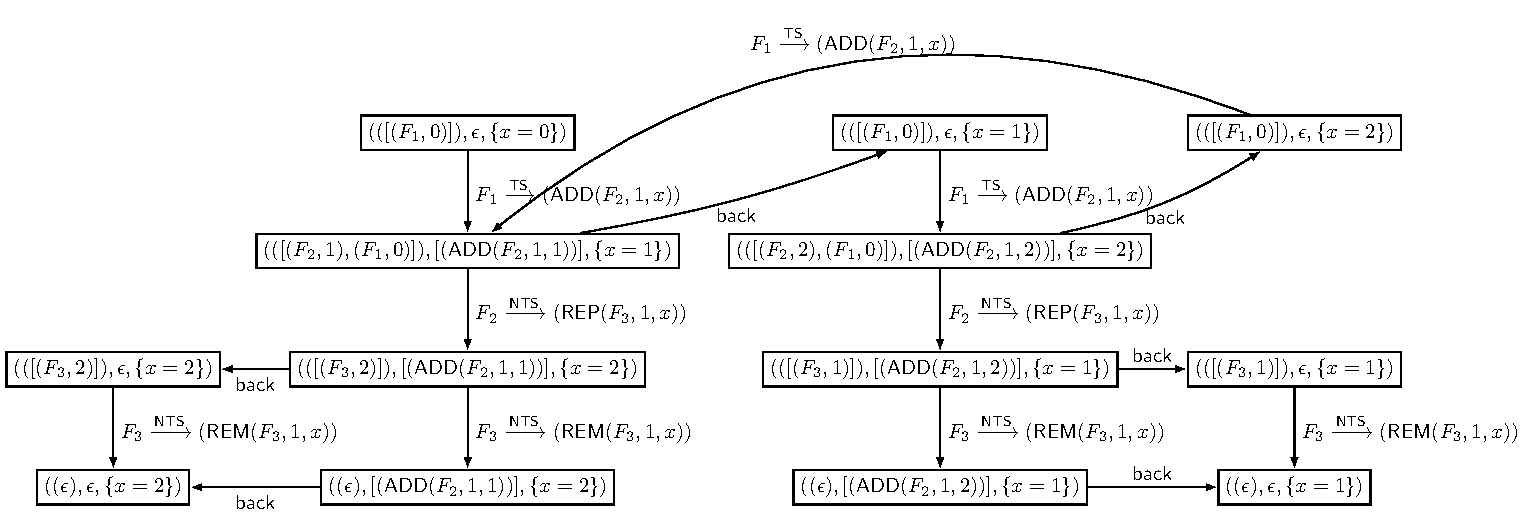
\includegraphics[scale = 0.6]{frg-example.pdf}
            \caption{Configurations that are reachable from the configuration $(([(F_1,0)]),\epsilon,\{x=0\})$ in $\Mm$}
                %in $\phi$
        % \vspace{-6mm}	
        \label{frg-example}
    \end{figure}


\end{example}
